\section*{Problem 1}
	\begin{proof} [Solution]
		The equation is:
		\begin{align}
			P(n, k + 1) = p_rP(n - 1, k) + p_lP(n + 1, k) + p_sP(n, k) \label{origin}
		\end{align}
		where $p_r, p_l, p_s$ are probabilities of moving right, left, and the same each. They satisfy $p_r + p_l + p_s = 1$. Suppose $p_r = p_l = p_s = \frac{1}{3}$. By Taylor expansion,
		\begin{align*}
			P(n, k + 1) &\simeq P(n, k) + P_k + \frac{1}{2}P_{kk} + \cdots\\
			P(n - 1, k) &\simeq P(n, k) - P_n + \frac{1}{2}P_{nn} - \cdots\\
			P(n + 1, k) &\simeq P(n, k) + P_n + \frac{1}{2}P_{nn} + \cdots
		\end{align*}
		Note that $\Delta k = \Delta n = 1$ in this discrete situation. By putting them into the equation (\ref{origin}), we get
		\begin{align*}
			P_k &\simeq \frac{1}{3}P_{nn}
		\end{align*}
		Therefore, the diffusion coefficient is $\frac{1}{3}$ if $\Delta k = \Delta n = 1$. If not, then the general version is $\frac{1}{3}\frac{{\Delta n}^2}{\Delta k}$. If we apply the similar analysis as we did in class, then we get the same result: $\mu(t) = 0, \sigma^2(t) = 2Dt$ where $D$ is a diffusion coefficient. However, since $D$ has decreased compared to two movement choices, $\sigma^2$ is further reduced. Here are the results.
		\begin{figure} [hbt!]
			\centering
			\subfloat[2-choice walk]{{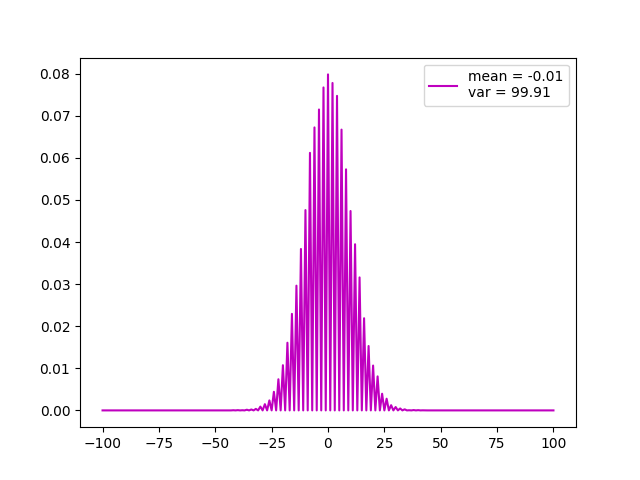
\includegraphics[width=0.4\textwidth]{2step_walk.png}}}
			\subfloat[3-choice walk]{{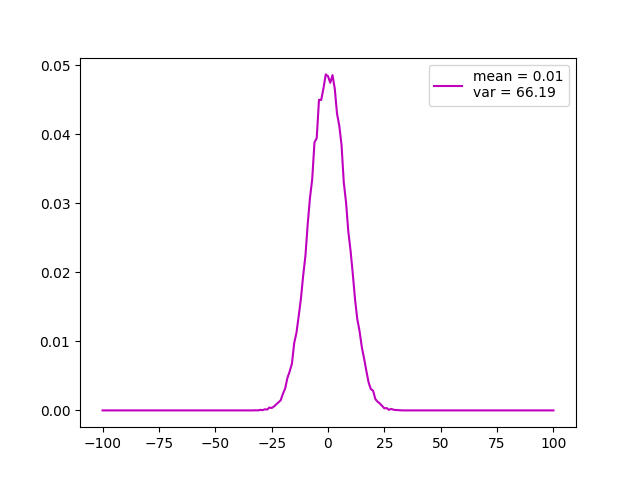
\includegraphics[width=0.4\textwidth]{3step_walk.png}}}
		\end{figure}\\
	\end{proof}